\documentclass[tikz,border=8pt]{standalone}
\usepackage{amsmath}
\usetikzlibrary{arrows.meta,positioning,fit}
\definecolor{blue}{HTML}{0072B2}\definecolor{red}{HTML}{D55E00}
\definecolor{green}{HTML}{009E73}\definecolor{ink}{HTML}{172033}
\definecolor{pale}{HTML}{F2F4F7}\definecolor{muted}{HTML}{667085}
\begin{document}
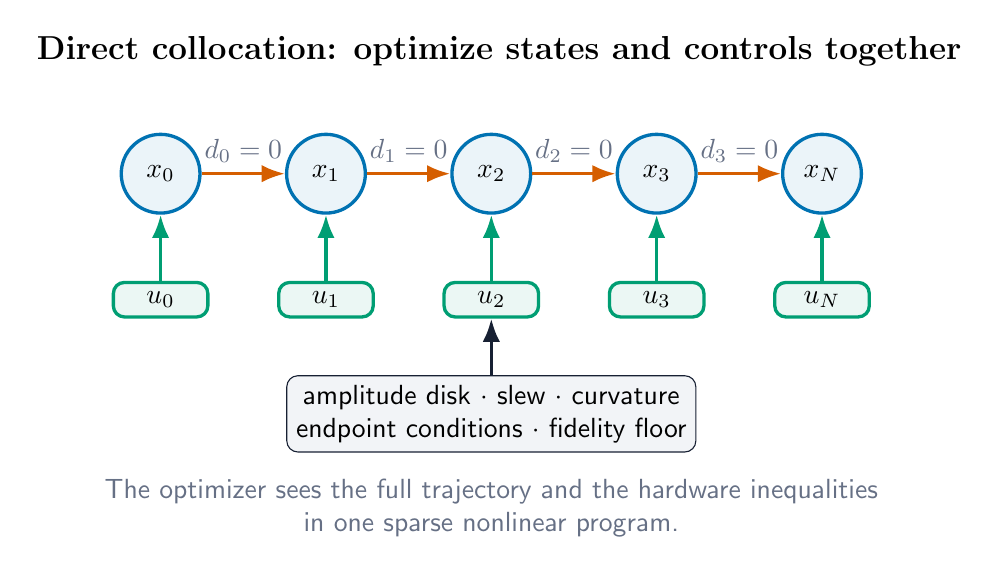
\begin{tikzpicture}[font=\sffamily,>=Latex]
  \node[font=\bfseries\large] at (4.3,3.35) {Direct collocation: optimize states and controls together};
  \foreach \x/\i in {0/0,2.1/1,4.2/2,6.3/3,8.4/N} {
    \node[circle,draw=blue,very thick,fill=blue!8,minimum size=10mm] (x\i) at (\x,1.8) {$x_{\i}$};
    \node[rounded corners,draw=green,very thick,fill=green!8,minimum width=12mm] (u\i) at (\x,.2) {$u_{\i}$};
    \draw[->,green,very thick] (u\i) -- (x\i);
  }
  \foreach \a/\b in {0/1,1/2,2/3,3/N} {
    \draw[->,red,very thick] (x\a) -- (x\b) node[midway,above,muted] {$d_{\a}=0$};
  }
  \node[draw=ink,rounded corners,fill=pale,align=center,minimum width=4.0cm] (constraints) at (4.2,-1.25) {amplitude disk $\cdot$ slew $\cdot$ curvature\\endpoint conditions $\cdot$ fidelity floor};
  \draw[->,ink,very thick] (constraints.north) -- (u2.south);
  \node[align=center,muted] at (4.2,-2.45) {The optimizer sees the full trajectory and the hardware inequalities\\in one sparse nonlinear program.};
\end{tikzpicture}
\end{document}
